\documentclass[12pt]{article}
\usepackage[margin=1in]{geometry}
\usepackage{graphicx}
\usepackage{hyperref}
\usepackage{float}
\usepackage{color}
\usepackage{enumitem}

\hypersetup{
    colorlinks,
    citecolor=black,
    filecolor=black,
    linkcolor=black,
    urlcolor=black
}

\title{RISC-V: A Didactic Platform \\
\large Documentation}

\author{Jules PERRIN, Professor: Theo Kluter}
\date{\today}

\begin{document}
\maketitle
\tableofcontents

\section{Introduction}
This document describes the RV32IM processor and its architecture. I've tried to make it as clear 
as possible such that everyone with a basic knowledge of computer architecture can understand it.
It will describe each significant module of the processor, what it does and what are the different
inputs and outputs with an image of the module. To avoid repeating too much the signal, I will only list 
the signals directly linked to the module, that's why most of the stages don't have any signals listed because 
it's their inside modules that are using them and will be listed here instead. \\

It is recommended to follow this document with the source code of the processor, which is available
in the Verilog folder of the project.
Don't hesitate to use the table of contents to navigate through the different parts of the document.
If you see any mistake or are confused by something don't hesitate to contact me at the mail address
\href{mailto:jules.perrin@epfl.ch}{jules.perrin@epfl.ch}.

\section{Fetch}
\subsection{IF Stage}

\begin{figure}[H]
\centering
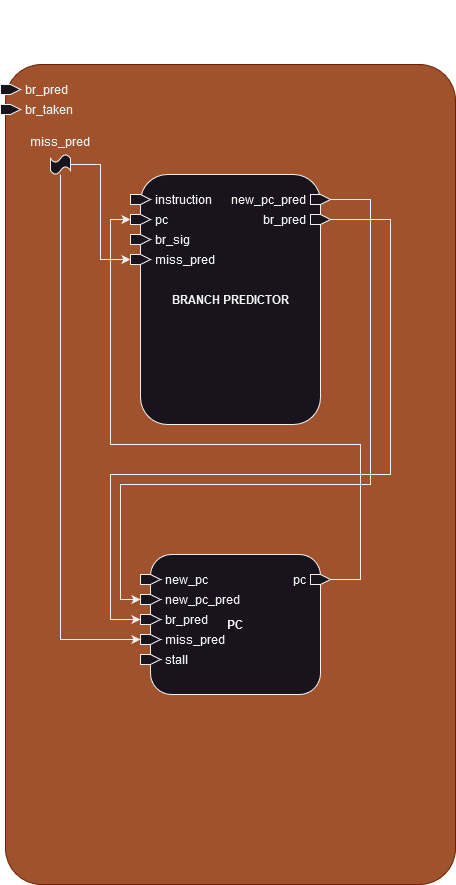
\includegraphics[width=0.5\textwidth]{../diagrams/fetch/if_stage.png}
\caption{Diagram of the IF Stage}
\label{fig:IF_Stage}
\end{figure}

The IF stage is responsible for fetching the next instruction from the ROM and passing it to the ID stage. 
The IF stage contains two different modules: the PC and the branch predictor.
The IF stage is the only stage that computes a value outside of a value, it uses the $br\_pred$ signal and the 
$br\_taken$ signal to compute if there is a miss prediction such that the PC and the branch predictor can be updated
accordingly. \\

Signals:
\begin{enumerate}
    \item Input: $br\_pred$, This signal is representing the state of the prediction made by the branch predictor in the EX stage.
    \item Input: $br\_taken$, This signal is representing the state of the branch in the EX stage.
    \item Output: $miss\_pred$, This signal is representing if there is a miss prediction or not.
\end{enumerate}

\subsection{Branch Predictor}

\begin{figure}[H]
\centering
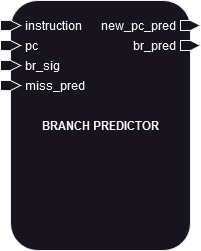
\includegraphics[width=0.5\textwidth]{../diagrams/fetch/br_predictor.png}
\caption{Diagram of the Branch Predictor}
\label{fig:br_predictor}
\end{figure}

The branch predictor as its name suggests is responsible for predicting if the branch will be taken or not. The algorithm that 
is being used is the two-level adaptive branch predictor, which I will not describe in detail but reuse the idea of a 
2-bit saturating counter but apply a bit of the notion of locality and pattern recognition. Of course, the algorithm
could be improved or replaced by any other algorithm and it is up to the user to do it if he wants to.
It works at the beginning by doing a simple matching on the current instruction to see if it is a branch instruction.
If that's the case we look if it is a conditional branch or not, if it is not we simply predict that the branch will be taken for 
the JAL instruction, but the JALR one will be always predicted as not taken for data dependency reasons. If it is a conditional branch
we simply use the algorithm described above to predict if the branch will be taken or not. The algorithm updates the prediction depending 
on the actual result of the branch that is represented by the $miss\_pred$ signal. If the prediction is taken, we compute the next PC \\

Signals:
\begin{enumerate}[label={\textbullet}]
    \item Input: $instruction$, This signal is representing the current instruction that is being fetched.
    \item Input: $pc$, This signal is representing the current PC.
    \item Input: $br\_sig$ This signal is representing the state of the current instruction in the EX stage. It is used to know if the instruction is a branch or not.
    such that it updates only the algorithm when it is a branch instruction.
    \item Input: $miss\_pred$, This signal is representing the state of the prediction made by the branch predictor in the EX stage.
    \item Output: $new\_pc\_pred$, This signal is representing the next PC that will be used if the prediction is taken.
    \item Output: $br\_pred$, This signal is indicating if the branch is predicted as taken or not.
\end{enumerate}

\subsection{PC}

\begin{figure}[H]
\centering
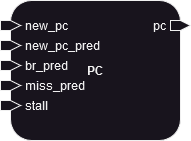
\includegraphics[width=0.5\textwidth]{../diagrams/fetch/pc.png}
\caption{Diagram of the PC}
\label{fig:PC}
\end{figure}

The PC is responsible for computing the next PC. It uses the different input signals to know which PC to compute.
for example, if it is a branch, the branch predictor will tell him what to do, and if the branch predictor is wrong
it will be updated accordingly. If it is a more classic instruction such as an ADD, it will simply increment the PC by 4
etc. \\

Signals:
\begin{enumerate}
    \item Input: $new\_pc$, This signal represent the next PC given by the branch unit in the EX stage.
    \item Input: $new\_pc\_pred$, This signal represent the next PC given by the branch predictor.
    \item Input: $br\_pred$, This signal is representing the state of the prediction made by the branch predictor in the EX stage.
    \item Input: $miss\_pred$, This signal is representing if there is a miss prediction or not.
    \item Input: $stall$, This signal is representing if the pipeline is stalled or not due to a data dependency in the ID stage.
    \item Output: $pc$, This signal is representing the current PC.
\end{enumerate}

\section{Decode}
\subsection{ID Stage}

\begin{figure}[H]
\centering
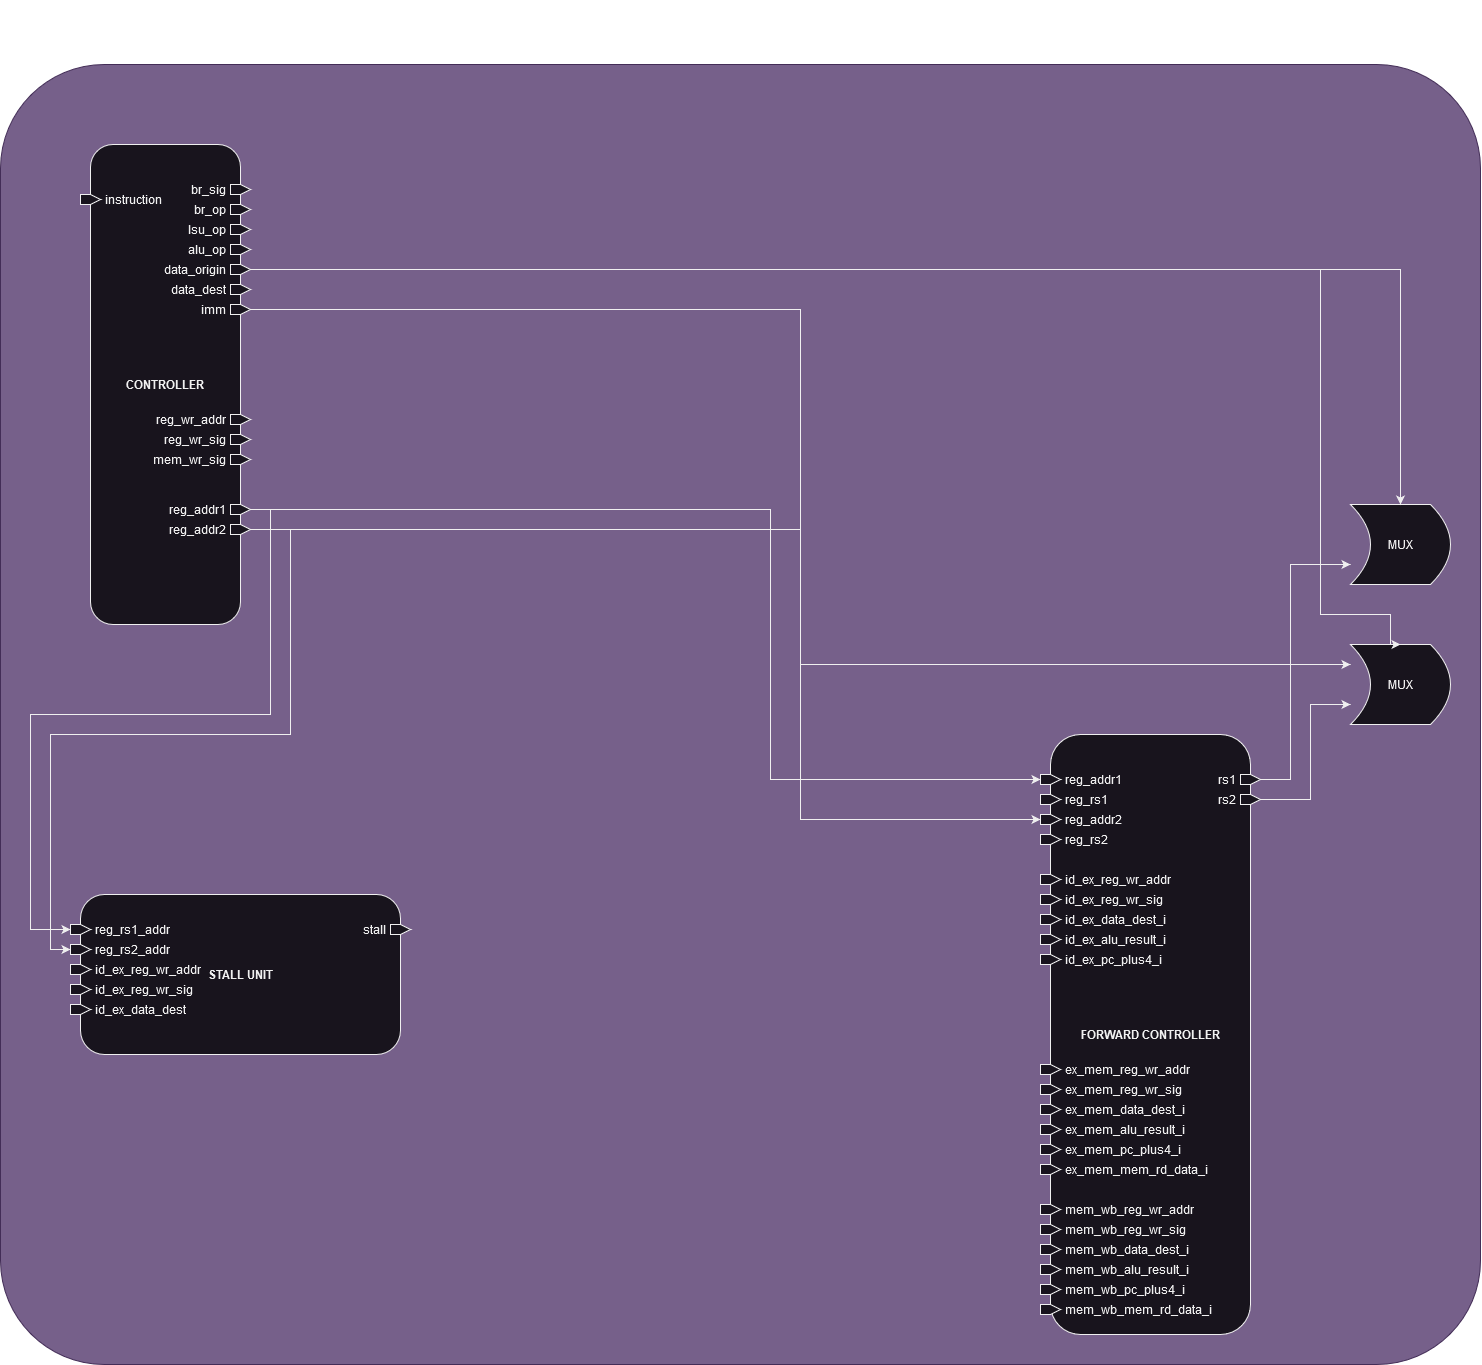
\includegraphics[width=1\textwidth]{../diagrams/decode/id_stage.png}
\caption{Diagram of the ID stage}
\label{fig:id_stage}
\end{figure}

The ID stage is the second stage of the pipeline. It is responsible for decoding the instruction and forwarding the data to the next stage. 
It is composed of the following modules: the controller which is the main module of the stage, the stall unit, the forward controller and 
2 smaller modules which are 2 muxes used to select between the different registers and the immediate value or the pc.





\subsection{Controller}

\begin{figure}[H]
\centering
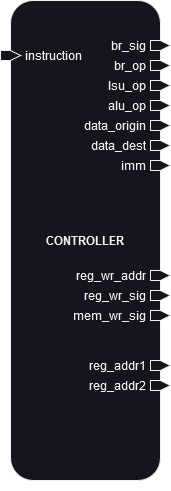
\includegraphics[width=0.35\textwidth]{../diagrams/decode/controller.png}
\caption{Diagram of the Controller}
\label{fig:controller}
\end{figure}

The controller is the main module of the ID stage. It is responsible for decoding the current instruction which is the action
of extracting the different fields of the instruction and forwarding them to the next stage. For more information about the different
types of instruction and how the data is encoded in the instruction, please refer to the RISC-V manual~\cite{riscv_manual}. \\

Signals:
\begin{enumerate}
    \item Input: $instruction$, This signal is representing the current instruction that is being decoded.
    \item Output: $br\_sig$, This signal is representing the state of the current instruction. 
    It is used to know if the instruction is a branch or not.
    \item Output: $br\_op$, This signal is representing the type of branch that is being executed.
    \item Output: $lsu_op$, This signal is representing the type of load or store that is being executed.
    \item Output: $alu\_op$, This signal is representing the type of ALU operation that is being executed.
    \item Output: $data\_origin$, This signal is representing the origin of the data that is being used by the ALU.
    That could be the registers, or one register and an immediate or one register and the PC.
    \item Output: $data\_dest$, This signal will be useful in the write-back stage to know which data to write back,
    so either the ALU result or the data from the memory or the next PC (so the PC+4).
    \item Output: $imm$, This signal is representing the immediate value that is being used by the ALU.
    \item Output: $reg\_wr\_addr$, This signal is representing the register address that will be written back.
    \item Output: $reg\_wr\_sig$, This signal is representing if we want to write to the register file or not.
    \item Output: $mem\_wr\_sig$, This signal is representing if we want to write to the memory or not.
    \item Output: $reg\_addr1$, This signal is representing the first register address that has been extracted from the instruction.
    \item Output: $reg\_addr2$, This signal is representing the second register address that has been extracted from the instruction.
\end{enumerate}
\paragraph{Stall Unit}

\begin{figure}[H]
    \centering
    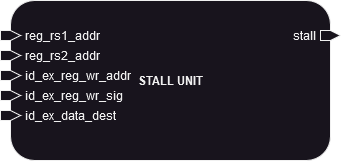
\includegraphics[width=0.5\textwidth]{design/pipelined/decode/images/stall_unit.png}
    \caption{Diagram of the Stall Unit}
    \label{fig:stall_unit}
\end{figure}

The stall unit is a small module that is used to stall the pipeline when a data dependency that cannot be resolved by forwarding is detected
which should only happen if we use the result of a load instruction in the next instruction. It is simply comparing the register addresses of the
current instruction with the register that is being written by the previous instruction. If there is a match, it looks what is the operation that is
being executed by the current instruction and if it is a load, it will stall the pipeline. \\

Signals:
\begin{enumerate}[label={\textbullet}]
    \item Input: $reg\_rs1\_addr$, This signal is representing the first register address that is being used by the current instruction.
    \item Input: $reg\_rs2\_addr$, This signal is representing the second register address that is being used by the current instruction.
    \item Input: $id\_ex\_reg\_wr\_addr$, This signal is representing the register address that is being written by the previous instruction.
    \item Input: $id\_ex\_reg\_wr\_sig$, This signal is representing if the previous instruction is written to the register file or not.
    It is used to differentiate between a load and a store.
    \item Input: $id\_ex\_data\_dest$, This signal is representing the origin of the data that is being used by the ALU in the previous instruction.
    In this case only if the previous instruction has a data dest of MEM then we need to stall the pipeline.
    \item Output: $stall$, This signal is representing if we need to stall the pipeline or not.
\end{enumerate}
\subsection{Forward Controller}

\begin{figure}[H]
\centering
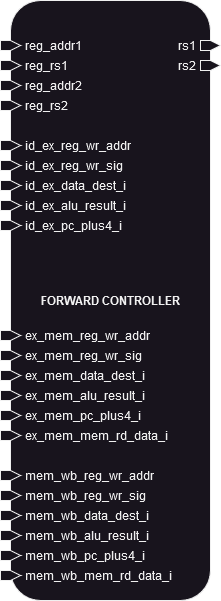
\includegraphics[width=0.35\textwidth]{../diagrams/decode/forward_controller.png}
\caption{Diagram of the Forward Controller}
\label{fig:forward_controller}
\end{figure}

The forward controller is a module that is used to control what are the values used as rs1 and rs2 in the ALU. 
For example, if you have a data dependency between two instructions, the first one is a load and the second one is an add,
you need to forward the result of the load to the ALU. This module is responsible for that and instead of using the value of the register file,
it will use the value that is being forwarded. \\

Signals:
\begin{enumerate}[label={\textbullet}]
    \item Input: $reg_addr1$, This signal is representing the first register address that is being used by the current instruction.
    \item Input: $reg_rs1$, This signal is representing the value of the first register that is being used by the current instruction.
    \item Input: $reg_addr2$, This signal is representing the second register address that is being used by the current instruction.
    \item Input: $reg_rs2$, This signal is representing the value of the second register that is being used by the current instruction.
    \item Input: $id\_ex\_reg\_wr\_addr$, This signal is representing the register address that is being written by the previous instruction.
    \item Input: $id\_ex\_reg\_wr\_sig$, This signal is representing if the previous instruction is written to the register file or not.
    \item Input: $id\_ex\_data\_dest$, This signal is representing the origin of the data that is being used by the ALU in the previous instruction.
    \item Input: $id\_ex\_alu\_result$, This signal is representing the result of the ALU in the previous instruction.
    \item Input: $id\_ex\_pc\_plus4$, This signal is representing the pc plus 4 of the previous instruction.
    \item Input: $ex\_mem\_reg\_wr\_addr$, This signal is representing the register address that is being written by the previous instruction.
    \item Input: $ex\_mem\_reg\_wr\_sig$, This signal is representing if the previous instruction is written to the register file or not.
    \item Input: $ex\_mem\_data\_dest$, This signal is representing the origin of the data that is being used by the ALU in the previous instruction.
    \item Input: $ex\_mem\_alu\_result$, This signal is representing the result of the ALU in the previous instruction.
    \item Input: $ex\_mem\_pc\_plus4$, This signal is representing the pc plus 4 of the previous instruction.
    \item Input: $ex\_mem\_mem\_rd\_data$, This signal is representing the data that is being read from the memory in the previous instruction.
    \item Input: $mem\_wb\_reg\_wr\_addr$, This signal is representing the register address that is being written by the previous instruction.
    \item Input: $mem\_wb\_reg\_wr\_sig$, This signal is representing if the previous instruction is written to the register file or not.
    \item Input: $mem\_wb\_data\_dest$, This signal is representing the origin of the data that is being used by the ALU in the previous instruction.
    \item Input: $mem\_wb\_alu\_result$, This signal is representing the result of the ALU in the previous instruction.
    \item Input: $mem\_wb\_pc\_plus4$, This signal is representing the pc plus 4 of the previous instruction.
    \item Input: $mem\_wb\_mem\_rd\_data$, This signal is representing the data that is being read from the memory in the previous instruction.
    \item Output: $rs1$, This signal is representing the value that should be used as rs1 in the ALU.
    \item Output: $rs2$, This signal is representing the value that should be used as rs2 in the ALU.
\end{enumerate}

\section{Toolchain}
I've also put as disposition an "easy" way to generate programs to use as input to the ROM of the processor. You still have to install 
the RISC-V toolchain to use it and configure correctly the bash or zsh file to indicate where the toolchain is installed.
Installing the toolchain can take quite a while since you'll have to compile it and can take more than 45min and will highly depend
on what CPU you have. \\

Here is a step-by-step guide to installing the toolchain:

\begin{enumerate}[label={\textbullet}]
    \item Clone the toolchain from \href{https://github.com/riscv-collab/riscv-gnu-toolchain}{here}.
    
    \begin{verbatim}
    git clone https://github.com/riscv/riscv-gnu-toolchain.git
    \end{verbatim}
    
    \item Navigate into the cloned directory.
    
    \begin{verbatim}
    cd riscv-gnu-toolchain
    \end{verbatim}
    
    \item Run the configuration script.

    \begin{verbatim}
    ./configure --prefix=/opt/riscv --with-arch=rv32im
    \end{verbatim}
    
    \item Compile the toolchain. This step may take a while.
    
    \begin{verbatim}
    make
    \end{verbatim}
    
    \item Once the compilation is done, add the toolchain to your PATH in your bash or zsh configuration file.

    \begin{verbatim}
    echo 'export PATH=$PATH:/opt/riscv/bin' >> ~/.bashrc
    source ~/.bashrc
    \end{verbatim}
\end{enumerate}

After that, you should be able to use the toolchain. To test it, you can try making a simple program like the ones in the 
$c\_code$ folder of the project. You can simply compile them with the following command:

\begin{verbatim}
    make
\end{verbatim}

That will generate a .hex file that you can use as input to the ROM of the processor. It will also give you the assembly
code of the program in the .s file so that you can see what the compiler generated. \\



\end{document}
